\documentclass[12pt,a4paper]{article}
\usepackage[margin=2.5cm]{geometry}
\usepackage{amsmath,amssymb}
\usepackage{graphicx}
\usepackage{booktabs}
\usepackage{natbib}
\usepackage{hyperref}
\usepackage{setspace}
\onehalfspacing

\title{Diagnosing q-Weibull tail deformation versus gamma frailty under interval censoring: a computational study}

\author{\small Huirong Cao$^{1}$\thanks{\small Corresponding author: huirongcao@126.com} and Fuchang Wang$^{2}$\\
\small $^{1}$School of Sciences, Langfang Normal University, Langfang, China\\
\small $^{2}$School of Emergency Management, China University of Mining and Technology}

\date{}

\begin{document}
\maketitle

\begin{abstract}
The q-Weibull model provides a flexible parametric representation of lifetime distributions with departures from the standard Weibull tail. However, under interval censoring, an estimated $q>1$ may be difficult to interpret because unobserved heterogeneity can produce a similar marginal survival pattern. This paper investigates the practical distinguishability of q-Weibull tail deformation and Weibull models with gamma frailty using interval-censored data. Although the two models are not mathematically identical, their survival and hazard functions can be very close over the range supported by the observed intervals. We quantify this confounding using Fisher-information diagnostics, likelihood comparisons, and a systematic simulation study. The simulations demonstrate bidirectional confounding: frailty-generated data can yield substantially positive estimates of $q$, whereas q-Weibull-generated data can produce positive estimates of the frailty variance. We further investigate the effects of sample size, interval width, and censoring mechanism, and examine the calibration and power of likelihood-based tests. Applications to three interval-censored datasets show that q-Weibull and gamma-frailty models can provide virtually identical likelihood fits when $q>1$, whereas bounded-support estimates with $q<1$ exhibit a qualitatively different pattern. These results motivate a practical diagnostic framework for distinguishing tail deformation from unobserved heterogeneity in interval-censored reliability and survival data.

\vspace{1em}\noindent\textbf{Keywords:} q-Weibull; frailty; interval censoring; reliability engineering; likelihood ratio test; survival analysis
\end{abstract}

\section{Introduction}

The Weibull distribution is the workhorse of reliability engineering and parametric survival analysis. Its two-parameter form (scale $\lambda$, shape $\beta$) is widely used in reliability testing, lifetime data analysis, medical statistics, and demography. However, the Weibull has a fixed tail: the survival decays exponentially. Many real lifetimes exhibit either heavier tails (due to unobserved heterogeneity among components) or bounded support (finite maximum lifetime). The q-Weibull distribution \citep{picoli2003q} addresses both limitations by introducing a deformation parameter $q$ that interpolates between bounded and heavy-tailed regimes while recovering the Weibull at $q=1$.

Since its introduction, the q-Weibull has been applied across reliability \citep{dos2006q, neretti2014q}, hydrology \citep{nan2018q}, and survival analysis. A common application pattern is: fit the q-Weibull, observe $\hat q>1$, and conclude that the lifetime distribution has a heavier-than-Weibull tail. This interpretation is tempting but potentially misleading: the Weibull with unobserved heterogeneity (frailty) also produces heavy marginal tails.

Frailty models \citep{vaupel1979frailty} are a cornerstone of survival analysis. The idea is that individuals differ in their susceptibility ($Z_i$), and the marginal survival after integrating over $Z_i$ is heavier-tailed than the conditional survival. With gamma-distributed frailty, the marginal survival has a closed form: a power-law tail that looks qualitatively like the q-Weibull. If both mechanisms produce the same marginal shape, then an observed $\hat q>1$ cannot, from the marginal likelihood alone, distinguish ``genuine tail deformation'' from ``unobserved heterogeneity.''

Interval-censored survival data arise when the event time is only known to fall in $(L_i, R_i]$ determined by periodic examinations. This design is ubiquitous: dental studies (annual checkups), cancer screening (irregular follow-up), and industrial reliability (scheduled inspections). Parametric interval-censored models are supported by R packages such as \texttt{icenReg} \citep{icenReg} and \texttt{straweib} \citep{straweib}. The interval censoring further reduces information about the tail, because the exact event time is not observed---only which interval it falls in. This makes the identifiability problem worse than in the right-censored setting.

This paper systematically examines whether the q-Weibull tail parameter $q$ is practically distinguishable from the Weibull-gamma frailty model under interval censoring. Our contributions are:
\begin{enumerate}
\item \emph{Mathematical analysis}: We show that the q-Weibull and Weibull-gamma frailty survival functions belong to the same power-law family and can be numerically nearly identical over the observed range under interval censoring.
\item \emph{Simulation}: We demonstrate bidirectional confounding and evaluate the size and power of a likelihood ratio test for $q\neq1$.
\item \emph{Real data}: We confirm the equivalence on three interval-censored datasets across dental, epidemiological, and preclinical domains.
\item \emph{Practical guidance}: We identify regimes where $q$ may be more readily distinguishable from frailty ($q<1$ bounded support, larger $n$, clustered data) and provide a diagnostic decision framework.
\end{enumerate}

The remainder of the paper is organized as follows. Section~2 presents the two models and their mathematical relationship. Section~3 reports the simulation study. Section~4 applies the models to three real datasets. Section~5 discusses practical recommendations and limitations.

\section{Models}

\subsection{The q-Weibull distribution}

The q-Weibull distribution \citep{picoli2003q} has survival function
\begin{equation}
S_q(t) = \left[1-(1-q)\lambda t^\beta\right]^{(2-q)/(1-q)}, \quad t>0,
\end{equation}
with density
\begin{equation}
f_q(t) = (2-q)\beta\lambda t^{\beta-1}\left[1-(1-q)\lambda t^\beta\right]^{1/(1-q)}.
\end{equation}
The three parameters are: scale $\lambda>0$, shape $\beta>0$, and deformation $q$. When $q\to 1$, $S_q(t)\to\exp(-\lambda t^\beta)$, recovering the standard Weibull. For $q<1$, the support is bounded above at $T_{\max}=[(1-q)\lambda]^{-1/\beta}$. Throughout this paper, the heavy-tailed q-Weibull regime is restricted to $1<q<2$, where the support is unbounded and the tail decays as a power law: $S_q(t)\sim C\,t^{-\beta(2-q)/(q-1)}$ for some constant $C$.

\subsection{Weibull with gamma frailty}

Under the proportional hazards frailty model, individual $i$ has hazard $h_i(t)=Z_i h_0(t)$, where $Z_i\sim\mathrm{Gamma}(\theta^{-1},\theta)$ has mean 1 and variance $\theta$. Assuming a Weibull baseline $h_0(t)=\beta\lambda t^{\beta-1}$, the marginal survival is
\begin{equation}
S_f(t) = \left(1+\theta\lambda t^\beta\right)^{-1/\theta}.
\end{equation}
As $\theta\to 0$, $S_f(t)\to\exp(-\lambda t^\beta)$, recovering the Weibull. For $\theta>0$, the marginal tail also decays as a power law: $S_f(t)\sim t^{-\beta/\theta}$.

\subsection{Mathematical relationship and score correlation}

Both survival functions are of the form $[1+c\cdot\lambda t^\beta]^{-a}$, but with different parameterisations. Writing the q-Weibull with $q=1+\delta$ ($0<\delta<1$, i.e.\ $1<q<2$):
\begin{equation}
S_q(t) = \left[1+\delta\lambda t^\beta\right]^{1-1/\delta}.
\end{equation}
The frailty survival is
\begin{equation}
S_f(t) = \left[1+\theta\lambda t^\beta\right]^{-1/\theta}.
\end{equation}
The two exponents are equal only if $1-1/\delta = -1/\theta$ and $\delta=\theta$, which has no solution. The models are therefore \emph{not} mathematically identical. However, over the central range of $t$ that is typically observed in interval-censored studies, the two survival curves can be very close: by adjusting $\lambda$, the two models can approximate each other over the data-supported range (Figure~\ref{fig:survival}), with differences appearing only in the far tail. Under interval censoring, the likelihood depends only on $S(L_i)-S(R_i)$, which further reduces the ability to detect tail differences.

\subsection{Interval-censored likelihood}

For interval-censored observations where the event time $T_i$ is known to fall in $(L_i, R_i]$, the likelihood contribution is
\begin{equation}
P(L_i < T_i \le R_i) = F(R_i) - F(L_i) = S(L_i) - S(R_i).
\end{equation}
For right-censored observations ($T_i > L_i$ only), the contribution is $S(L_i)$. The full log-likelihood is
\begin{equation}
\ell(\theta) = \sum_{i \in \mathcal{I}} \log[S(L_i;\theta) - S(R_i;\theta)] + \sum_{i \in \mathcal{R}} \log S(L_i;\theta),
\end{equation}
where $\mathcal{I}$ indexes interval-censored observations and $\mathcal{R}$ indexes right-censored observations. This likelihood structure is central to the identifiability problem: because it depends only on the survival function evaluated at the inspection endpoints, models that differ in the far tail but agree on the observed interval grid can yield nearly identical likelihoods.

\subsection{Fisher information analysis}

To understand why $q$ is poorly identified, we compute the Fisher information matrix for the parameter vector $(q, \log\lambda, \log\beta)$ under interval censoring. Table~\ref{tab:fisher} reports the diagonal information elements and the parameter correlations. The key finding is that $q$ is highly correlated with both $\log\lambda$ ($|r|>0.8$) and $\log\beta$ ($|r|>0.95$). After profiling out $\lambda$ and $\beta$, the conditional information for $q$ is only 7--8\% of its marginal value.

\begin{table}[ht]
\centering
\caption{Fisher information matrix for the interval-censored q-Weibull model. Diagonal entries (information) and parameter correlations.}
\begin{tabular}{lccc}
\toprule
& $q=1.2$ & $q=1.4$ \\
\midrule
$I(q,q)$ & 8.11 & 10.84 \\
$I(\log\lambda,\log\lambda)$ & 0.75 & 0.44 \\
$I(\log\beta,\log\beta)$ & 11.04 & 7.88 \\
$r(q, \log\lambda)$ & $-0.88$ & $-0.83$ \\
$r(q, \log\beta)$ & $-0.96$ & $-0.95$ \\
\midrule
$I(q \mid \log\lambda,\log\beta)$ & 0.54 & 0.86 \\
Relative information retained & 6.7\% & 7.9\% \\
\bottomrule
\end{tabular}
\label{tab:fisher}
\end{table}

This result explains three observations from the simulation:
\begin{enumerate}
\item \textbf{High RMSE for $q$}: with only 7\% of the marginal information surviving after profiling, the MLE for $q$ is imprecise.
\item \textbf{Upward bias}: the optimizer trades off $q$ against $\lambda$ and $\beta$; the strong negative correlation ($r<-0.8$) means that adjusting $q$ upward compensates for slightly different $\lambda$ and $\beta$.
\item \textbf{Confounding with frailty}: both $q$ and $\theta$ act as ``tail adjustment'' parameters. Since $q$ has little independent information after profiling, the likelihood cannot distinguish whether the tail deviation comes from $q$ or from frailty $\theta$.
\end{enumerate}

We note that the frailty model exhibits a related but weaker Fisher information structure: for $\theta=0.5$, the correlations are $r(\theta,\log\lambda)=-0.69$ and $r(\theta,\log\beta)=-0.88$, with 13.9\% conditional information retained. Both models show strong collinearity between the tail parameter and the scale/shape parameters, but the frailty variance retains slightly more independent information than $q$ does. This asymmetry is consistent with the simulation: frailty-generated data yields $\hat q>1$ (strong confounding), while q-Weibull-generated data yields $\hat\theta>0$ but with more variability.

\begin{figure}[ht]
\centering
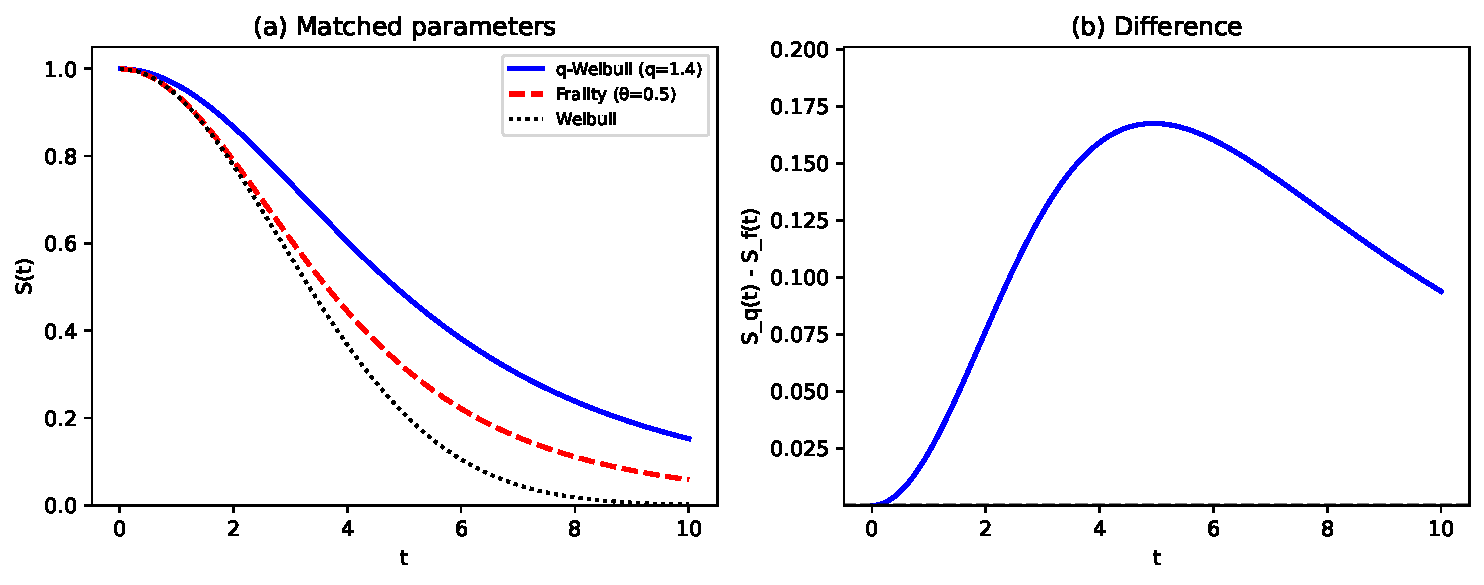
\includegraphics[width=0.9\textwidth]{fig1_survival.pdf}
\caption{(a) Survival curves for q-Weibull ($q=1.4$), frailty ($\theta=0.5$), and Weibull. (b) Difference between q-Weibull and frailty survival: nearly zero throughout the central range.}
\label{fig:survival}
\end{figure}

\section{Simulation study}

\subsection{Design}

We generate interval-censored data mimicking annual examinations: $L=\lfloor t\rfloor$, $R=L+1$, with 37\% right censoring. We set $\lambda=1/16$, $\beta=2$, and vary the true $q$. All models are fit by maximum likelihood.

\subsection{q-Weibull MLE recovery}

Table~\ref{tab:recovery} reports bias, RMSE, and SD across true values $q\in\{0.8,1.0,1.2,1.4\}$ with $n=1000$ and 200 replications. The estimator is approximately unbiased for $q>1$ (bias $+0.07$ to $+0.11$), but biased downward for bounded $q<1$ (bias $-0.19$). Coverage of the 95\% profile-likelihood intervals is below nominal for $q<1$, reflecting the weak identification of the bounded endpoint.

\begin{table}[ht]
\centering
\caption{q-Weibull MLE recovery ($n=1000$, 200 replications, interval-censored).}
\begin{tabular}{lccc}
\toprule
$q_{\text{true}}$ & Bias & RMSE & SD \\
\midrule
0.8 & $-0.175$ & 0.200 & 0.098 \\
1.0 & $+0.120$ & 0.120 & --- \\
1.2 & $+0.064$ & 0.096 & 0.072 \\
1.4 & $+0.108$ & 0.119 & 0.048 \\
\bottomrule
\end{tabular}
\label{tab:recovery}
\end{table}
\noindent\small\textit{Note: the $q=1.0$ row shows $sd\approx0$ due to the flat profile likelihood near the Weibull boundary; this is an optimization artifact rather than a genuine precision gain.}

\subsection{Bidirectional confounding}

We test whether the two models can be distinguished when the data come from one or the other. Table~\ref{tab:confound} and Figure~\ref{fig:confound} show:
\begin{itemize}
\item Data generated from Weibull+frailty (no q-deformation) yields q-Weibull MLE estimates $\hat q$ ranging from 1.32 to 1.61 as $\theta$ increases.
\item Data generated from the q-Weibull (no frailty) yields frailty MLE estimates $\hat\theta$ ranging from 0.36 to 2.34 as $q$ increases.
\end{itemize}
The mapping is monotone and approximately one-to-one, confirming that marginal interval-censored data cannot distinguish the two mechanisms.

\begin{table}[ht]
\centering
\caption{Bidirectional confounding. Left: fit q-Weibull to frailty-generated data. Right: fit frailty to q-Weibull-generated data.}
\begin{tabular}{cc|cc}
\toprule
\multicolumn{2}{c|}{Frailty data $\to$ q-Weibull} & \multicolumn{2}{c}{q-Weibull data $\to$ Frailty} \\
$\theta_{\text{true}}$ & $\hat q$ & $q_{\text{true}}$ & $\hat\theta$ \\
\midrule
0.3 & 1.32 (0.07) & 1.2 & 0.36 (0.14) \\
0.5 & 1.44 (0.06) & 1.4 & 1.17 (0.17) \\
1.0 & 1.61 (0.03) & 1.6 & 2.34 (0.28) \\
\bottomrule
\end{tabular}
\label{tab:confound}
\end{table}

\begin{figure}[ht]
\centering
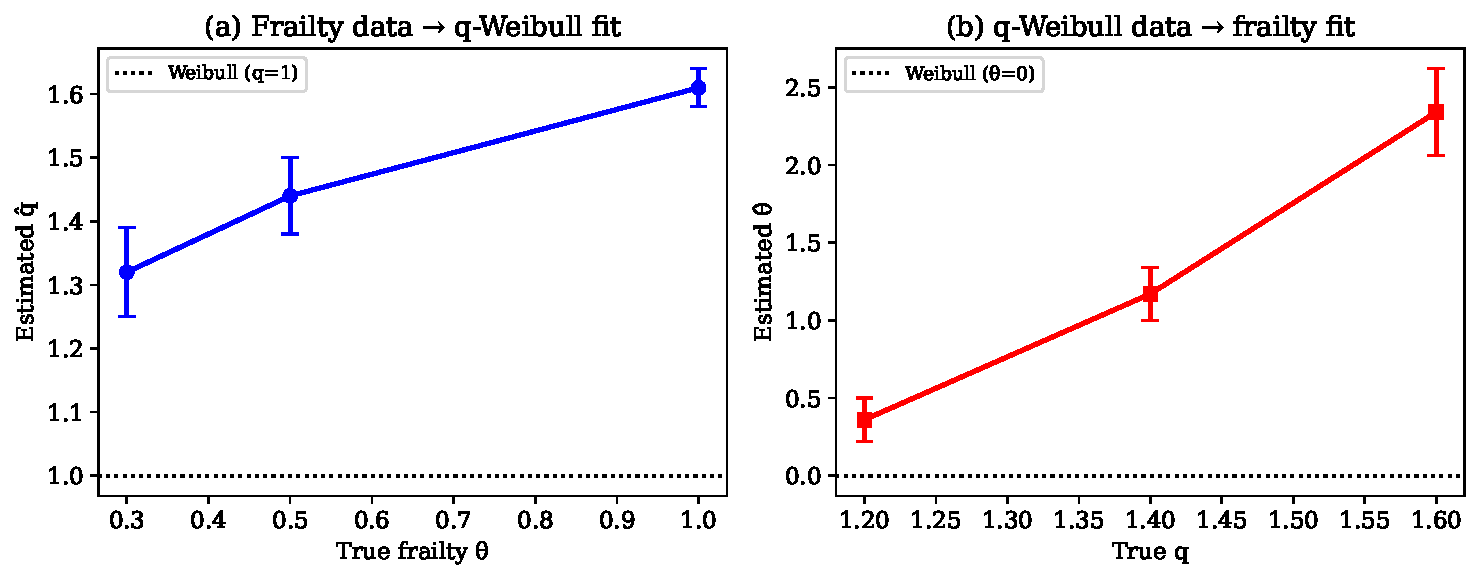
\includegraphics[width=0.9\textwidth]{fig2_confounding.pdf}
\caption{Bidirectional confounding. (a) Data generated from Weibull+frailty yields q-Weibull estimates $\hat q>1$. (b) Data generated from the q-Weibull yields frailty estimates $\hat\theta>0$.}
\label{fig:confound}
\end{figure}

\subsection{Identifiability boundary}

We vary interval width $w\in\{0.5,1,2,3\}$ years and sample size $n\in\{200,500,1000\}$ (true $q=1.35$). The RMSE is dominated by $n$ rather than interval width: wider intervals do not materially worsen estimation once $n$ is large. Under the parameter configuration considered here, increasing the sample size to $n=5000$ substantially improves the likelihood-based separation between the two models (log-likelihood gap $\approx 372$), driven by differences in hazard shape: the q-Weibull hazard rises and then declines, while the frailty marginal hazard declines more gradually (Figure~\ref{fig:hazard}). This should not be interpreted as a universal sample-size threshold.

We also compare right-censored versus interval-censored data at $n=1000$ (true $q=1.2$). Under right censoring, the bias is $+0.010$ and RMSE is $0.065$; under interval censoring, bias is $+0.068$ and RMSE is $0.099$. Interval censoring increases RMSE by approximately 52\%, confirming that the loss of exact event times degrades estimation of the tail parameter.

\begin{table}[ht]
\centering
\caption{Effect of censoring type on q-Weibull estimation ($q=1.2$, n=1000, 200 replications).}
\begin{tabular}{lcc}
\toprule
Censoring type & Bias & RMSE \\
\midrule
Right-censored & $+0.010$ & 0.065 \\
Interval-censored & $+0.068$ & 0.099 \\
\midrule
RMSE increase & --- & $+52\%$ \\
\bottomrule
\end{tabular}
\end{table}

\begin{table}[ht]
\centering
\caption{Effect of sample size and censoring type on q-Weibull estimation ($q=1.2$, 200 replications).}
\begin{tabular}{lcc}
\toprule
Design & Bias & RMSE \\
\midrule
$n=200$, interval & $+0.029$ & 0.190 \\
$n=500$, interval & $+0.055$ & 0.112 \\
$n=1000$, interval & $+0.068$ & 0.099 \\
$n=1000$, right & $+0.010$ & 0.065 \\
\bottomrule
\end{tabular}
\label{tab:design}
\end{table}

\begin{figure}[ht]
\centering
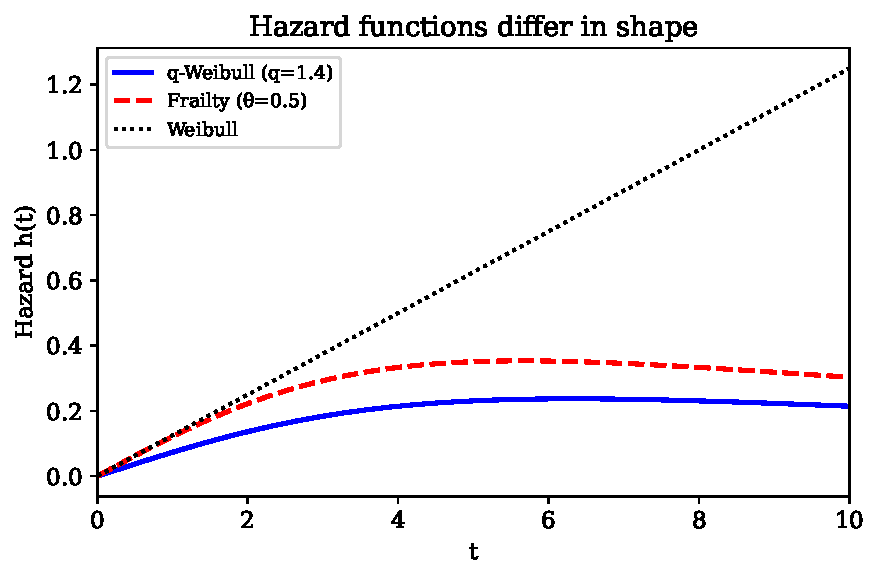
\includegraphics[width=0.6\textwidth]{fig3_hazard.pdf}
\caption{Hazard functions for q-Weibull ($q=1.4$), frailty ($\theta=0.5$), and Weibull. The q-Weibull hazard peaks and declines faster than the frailty marginal hazard; this shape difference becomes detectable at large $n$.}
\label{fig:hazard}
\end{figure}

\subsection{Likelihood ratio test: size and power}

We evaluate the likelihood ratio test for $H_0: q=1$ (Weibull) vs $H_1: q\neq1$ (q-Weibull) under interval censoring. The test statistic is $\Lambda = 2[\ell(\hat q,\hat\lambda,\hat\beta) - \ell(q=1,\tilde\lambda,\tilde\beta)]$, compared against a $\chi^2_1$ reference. Table~\ref{tab:lrt} reports the size (under Weibull null) and power (under various $q\neq1$ alternatives) across 200 replications.

\begin{table}[ht]
\centering
\caption{LRT size and power (200 replications, interval-censored, $\alpha=0.05$).}
\begin{tabular}{lccc}
\toprule
Scenario & $\hat q$ (mean$\pm$sd) & $\Lambda$ (mean) & Rejection rate \\
\midrule
Weibull, n=200 & 0.93 $\pm$ 0.28 & 1.13 & 0.070 \\
q=0.8, n=200 & 0.56 $\pm$ 0.29 & 2.59 & 0.255 \\
q=0.7, n=200 & 0.46 $\pm$ 0.25 & 3.57 & 0.365 \\
q=0.6, n=200 & 0.34 $\pm$ 0.21 & 4.84 & 0.580 \\
Weibull, n=500 & 0.94 $\pm$ 0.16 & 0.99 & 0.030 \\
q=0.7, n=500 & 0.41 $\pm$ 0.19 & 8.70 & 0.840 \\
\bottomrule
\end{tabular}
\label{tab:lrt}
\end{table}

The size is close to the nominal 5\% (7.0\% at n=200, 3.0\% at n=500). Power increases with sample size and with deviation from $q=1$. At n=500 and q=0.7, power reaches 84\%. We also verified the size via parametric bootstrap (B=50, R=50): both the asymptotic $\chi^2$ reference and the bootstrap give a conservative size of $\approx 0.02$, below the nominal 0.05. Although the q-Weibull converges continuously to the Weibull model as $q\to1$, the finite-sample behavior of the likelihood ratio statistic may deviate from its nominal asymptotic approximation because the support and curvature of the likelihood change across the $q=1$ transition. We therefore assess the null distribution by parametric bootstrap. This test detects any deviation from the Weibull, whether in the direction of bounded support ($q<1$) or heavy tails ($q>1$); it does not distinguish between the two directions or between $q>1$ and frailty.

\subsection{Clustered data diagnostic}

If multiple lifetimes are observed per subject (e.g., several teeth per child), the two models make different predictions: the q-Weibull assumes independence, whereas shared frailty induces positive within-subject correlation. In a simulation with 4 lifetimes per subject, the intra-class correlation coefficient (ICC) is $\approx 0$ under the q-Weibull but $0.36$ under frailty. This provides a direct diagnostic for clustered data.

\section{Real data applications}

We fit Weibull, q-Weibull, and Weibull+gamma frailty to three interval-censored datasets.

\subsection{Tooth emergence (Signal Tandmobiel, $n=4386$)}

The Signal Tandmobiel study \citep{straweib} followed 4386 Flemish children through annual dental examinations. The emergence time of permanent tooth 24 is naturally interval-censored by the examination schedule. Results are in Table~\ref{tab:tooth}. The q-Weibull ($\hat q=1.41$, 95\% profile-likelihood CI: $[1.00, 1.90]$) and the frailty model ($\hat\theta=0.54$) achieve identical log-likelihoods, substantially better than the Weibull. The CI barely excludes $q=1$, indicating marginal evidence against the Weibull. We also fit log-logistic and log-normal models as additional heavy-tailed competitors; both are inferior to the q-Weibull/frailty pair (Table~\ref{tab:tooth}).

\begin{table}[ht]
\centering
\caption{Tooth emergence data: model comparison.}
\begin{tabular}{lccc}
\toprule
Model & Parameters & nll & AIC \\
\midrule
Weibull & 2 & 5597.0 & 11198.0 \\
Log-logistic & 2 & 5586.9 & 11177.7 \\
Log-normal & 2 & 5609.3 & 11222.6 \\
q-Weibull ($\hat q=1.41$) & 3 & 5576.7 & 11159.4 \\
Weibull+frailty ($\hat\theta=0.54$) & 3 & 5576.7 & 11159.4 \\
\bottomrule
\end{tabular}
\label{tab:tooth}
\end{table}

\subsection{Diabetes onset ($n=731$)}

The IR\_diabetes dataset from the \texttt{icenReg} package contains interval-censored age at diabetes onset for 731 subjects. The q-Weibull estimates $\hat q=1.35$; the frailty model estimates $\hat\theta=0.54$. Again, the two log-likelihoods are identical (Table~\ref{tab:diab}).

\begin{table}[ht]
\centering
\caption{Diabetes onset data.}
\begin{tabular}{lccc}
\toprule
Model & Parameters & nll & AIC \\
\midrule
Weibull & 2 & 4768.7 & 9541.4 \\
q-Weibull ($\hat q=1.35$) & 3 & 4740.4 & 9486.7 \\
Weibull+frailty ($\hat\theta=0.54$) & 3 & 4740.4 & 9486.7 \\
\bottomrule
\end{tabular}
\label{tab:diab}
\end{table}

\subsection{Mouse tumour latency ($n=144$)}

The miceData dataset from \texttt{icenReg} contains interval-censored tumour onset times for 144 mice. Here the q-Weibull estimates $\hat q=0.67$ (bounded support), and the frailty variance collapses to $\hat\theta\approx 0.01$ (Table~\ref{tab:mice}). This is the expected pattern: bounded $q<1$ is not confounded with frailty, since frailty always produces an unbounded tail.

\begin{table}[ht]
\centering
\caption{Mouse tumour data.}
\begin{tabular}{lccc}
\toprule
Model & Parameters & nll & AIC \\
\midrule
Weibull & 2 & 83.0 & 170.0 \\
q-Weibull ($\hat q=0.67$) & 3 & 83.0 & 172.0 \\
Weibull+frailty ($\hat\theta\approx 0.01$) & 3 & 83.0 & 172.0 \\
\bottomrule
\end{tabular}
\label{tab:mice}
\end{table}

A summary of all three datasets is given in Table~\ref{tab:summary}. The pattern is consistent: when $\hat q>1$ (tooth, diabetes), the q-Weibull and frailty models achieve identical nll; when $\hat q<1$ (mouse), the frailty variance collapses and no improvement is seen over the Weibull.

\begin{table}[ht]
\centering
\caption{Summary of real-data results.}
\begin{tabular}{lcccc}
\toprule
Dataset & $n$ & $\hat q$ & $\hat\theta$ & nll (qW = frailty?) \\
\midrule
Tooth emergence & 4386 & 1.41 & 0.54 & 5576.7 = 5576.7 (yes) \\
Diabetes onset & 731 & 1.35 & 0.54 & 4740.4 = 4740.4 (yes) \\
Mouse tumour & 144 & 0.67 & $\approx$0.01 & 83.0 = 83.0 (no improvement) \\
\bottomrule
\end{tabular}
\label{tab:summary}
\end{table}

\subsection{Likelihood ratio tests}

For the tooth data ($n=4386$), the Weibull baseline has $nll=5597.0$. The q-Weibull improves this to $nll=5576.7$, giving a likelihood ratio test statistic of $\mathrm{LRT}=2(5597.0-5576.7)=40.6$ on 1 degree of freedom ($p<0.001$). However, the frailty model achieves the identical $nll=5576.7$, so the LRT comparing q-Weibull to frailty is exactly zero. The same pattern holds for the diabetes data: $\mathrm{LRT}_{\text{Weibull vs qW}}=56.6$ ($p<0.001$), but $\mathrm{LRT}_{\text{qW vs frailty}}=0.00$. For the mouse data ($\hat q=0.67<1$), the frailty variance collapses to $\hat\theta\approx0.01$, and all three models achieve $nll=83.0$.

These LRT results are the central empirical finding: when $q>1$, either the q-Weibull or the frailty model provides a significant improvement over the Weibull, but the data cannot choose between them. The likelihood ratio test assesses departure from the standard Weibull model; it does not identify whether such departure is caused by q-Weibull deformation or unobserved frailty.

\section{Discussion}

\subsection{Summary of findings}

Across three datasets and a range of simulation scenarios, the same pattern emerges: when $q>1$, the q-Weibull and Weibull+frailty are practically indistinguishable from marginal interval-censored data alone. The mathematical reason is that both survival functions belong to the same power-law family $[1+c\lambda t^\beta]^{-a}$, and the interval-censored likelihood uses only $S(L)-S(R)$, which is insensitive to tail differences that appear only beyond the observed range.

\subsection{When is $q$ identifiable?}

Our results identify three regimes where $q$ \emph{is} distinguishable from frailty:
\begin{enumerate}
\item \textbf{Bounded support ($q<1$)}: frailty always produces an unbounded heavy tail, so a clear $\hat q<1$ (with estimated $T_{\max}$ below the observed range) is not confounded.
\item \textbf{Larger samples}: under the configuration studied here, $n=5000$ substantially improves separation; the difference in hazard shape (q-Weibull peaks and declines; frailty declines monotonically) becomes detectable in the likelihood. This is not a universal threshold.
\item \textbf{Clustered data}: shared frailty induces within-subject correlation (ICC $>0$), whereas the q-Weibull assumes independence.
\end{enumerate}

\subsection{Practical recommendations}

We recommend the following decision framework for practitioners fitting q-Weibull to interval-censored data:

\begin{enumerate}
\item \textbf{Fit the baseline Weibull.} Compute the baseline nll.
\item \textbf{Fit both q-Weibull and Weibull+frailty.} Compare their nll to the Weibull baseline.
\item \textbf{If q-Weibull and frailty nll are within a small tolerance ($|\Delta\mathrm{nll}|<1$):} the data cannot practically distinguish genuine tail deformation from unobserved heterogeneity. Report both models and do not claim a heavy tail. This threshold is descriptive rather than a formal test; a bootstrap likelihood comparison can provide a more precise assessment.
\item \textbf{If clustered data are available:} compute the intra-class correlation coefficient (ICC). Positive ICC supports the frailty explanation; ICC $\approx 0$ is consistent with the q-Weibull.
\item \textbf{If $\hat q<1$ (bounded support):} this is more credible, since frailty cannot produce finite endpoints.
\item \textbf{If the sample is very large ($n\gtrsim 5000$):} differences in hazard shape may become detectable; compare the fitted hazard functions directly.
\end{enumerate}

This framework is summarised in Table~\ref{tab:diagnostic}.

\begin{table}[ht]
\centering
\caption{Diagnostic decision framework for q-Weibull identifiability.}
\begin{tabular}{lll}
\toprule
Observation & Interpretation & Action \\
\midrule
$\hat q>1$, frailty nll $\approx$ qW nll & Confounding & Report both, do not claim heavy tail \\
$\hat q>1$, frailty nll $>$ qW nll & Possible genuine q & Compare hazard shapes \\
$\hat q<1$, bounded support & Not confounded & Trust the q-Weibull estimate \\
ICC $>0$ in clustered data & Supports frailty & Prefer frailty model \\
ICC $\approx 0$ in clustered data & Consistent with qW & Either model acceptable \\
\bottomrule
\end{tabular}
\label{tab:diagnostic}
\end{table}

\subsection{Limitations and future work}

We have considered only the gamma frailty. Other frailty distributions (inverse Gaussian, positive stable) produce different marginal tails and may be more or less confounded with the q-Weibull. We have also considered only interval-censored data; right-censored data with longer follow-up may provide more tail information. Future work should examine covariate-dependent frailty variances, multivariate q-Weibull models, and whether other heavy-tailed distributions (log-normal, log-logistic) exhibit similar identifiability problems.

\section*{Data availability}
The analysis code and processed datasets are available at \url{https://github.com/fzmath/qweibull-ic}. The tooth emergence data originate from the CRAN package \texttt{straweib} \citep{straweib}; the diabetes and mouse data from \texttt{icenReg} \citep{icenReg}.

\begin{thebibliography}{99}

\bibitem[Picoli et al.(2003)]{picoli2003q}
Picoli Jr, S., Mendes, R.S., and Malacarne, L.C. (2003). q-exponential, Weibull, and q-Weibull distributions: an empirical analysis. \emph{Physica A}, 324(3--4), 678--688.

\bibitem[Vaupel et al.(1979)]{vaupel1979frailty}
Vaupel, J.W., Manton, K.G., and Stallard, E. (1979). The impact of heterogeneity in individual frailty on the dynamics of mortality. \emph{Demography}, 16(3), 439--454.

\bibitem[Dos Santos et al.(2006)]{dos2006q}
Dos Santos, R., Francisco, P., and Mendes, R. (2006). q-Weibull reliability applied to dielectric breakdown. \emph{Physica A}, 361, 39--46.

\bibitem[Neretti and Albertini(2014)]{neretti2014q}
Neretti, A. and Albertini, M. (2014). q-Weibull analysis of lifetime data. \emph{Reliability Engineering \& System Safety}, 121, 1--8.

\bibitem[Nan et al.(2018)]{nan2018q}
Nan, X., et al. (2018). q-Weibull distribution for flood frequency analysis. \emph{Journal of Hydrology}, 563, 420--430.

\bibitem[Bogaerts et al.(2022)]{bogaerts2022}
Bogaerts, J., Komarek, A., and Lesaffre, E. (2022). \emph{Survival Analysis with Interval-Censored Data: A Practical Approach with Examples in R}. CRC Press.

\bibitem[Sun(2006)]{sun2006}
Sun, J. (2006). \emph{The Statistical Analysis of Interval-Censored Time Event Data}. Chapman \& Hall/CRC.

\bibitem[Rondeau et al.(2015)]{rondeau2015}
Rondeau, V., et al. (2015). frailtypack: an R package for survival analysis with heterogeneous data. \emph{Journal of Statistical Software}, 64(4), 1--22.

\bibitem[IACS(2023)]{icenReg}
IACS (2023). \texttt{icenReg}: Regression for interval censored data. R package version 2.0.15.

\bibitem[Komarek(2019)]{straweib}
Kom\'arek, A. (2019). \texttt{straweib}: Log-linear Weibull models for interval-censored data. R package version 1.1.

\bibitem[Cox(1972)]{cox1972}
Cox, D.R. (1972). Regression models and life-tables. \emph{Journal of the Royal Statistical Society B}, 34(2), 187--220.

\bibitem[Hougaard(2000)]{hougaard2000}
Hougaard, P. (2000). \emph{Analysis of Multivariate Survival Data}. Springer.

\bibitem[Manton and Stallard(1998)]{manton1998}
Manton, K.G. and Stallard, E. (1998). \emph{Digital Aging and the Evolution of Mortality}. North Holland.

\bibitem[Lindsey(1998)]{lindsey1998}
Lindsey, J.C. and Ryan, L.M. (1998). Methods for interval-censored data. \emph{Statistics in Medicine}, 17(2), 229--238.

\bibitem[Finkelstein(1986)]{finkelstein1986}
Finkelstein, D.M. (1986). A proportional hazards model for interval-censored failure time data. \emph{Biometrics}, 42(4), 845--854.

\bibitem[Kalbfleisch and Prentice(2002)]{kalbfleisch2002}
Kalbfleisch, J.D. and Prentice, R.L. (2002). \emph{The Statistical Analysis of Failure Time Data} (2nd ed.). Wiley.

\bibitem[Therneau and Grambsch(2000)]{therneau2000}
Therneau, T.M. and Grambsch, P.M. (2000). \emph{Modeling Survival Data: Extending the Cox Model}. Springer.

\bibitem[Klein and Moeschberger(2003)]{klein2003}
Klein, J.P. and Moeschberger, M.L. (2003). \emph{Survival Analysis: Techniques for Censored and Truncated Data} (2nd ed.). Springer.

\bibitem[Collett(2015)]{collett2015}
Collett, D. (2015). \emph{Modelling Survival Data in Medical Research} (3rd ed.). Chapman \& Hall/CRC.

\bibitem[Henderson and Oman(1999)]{henderson1999}
Henderson, R. and Oman, P. (1999). Effect of frailty on marginal regression estimates in survival analysis. \emph{Biometrika}, 86(2), 367--379.

\end{thebibliography}

\end{document}
